% --------------------------
% Document class
% --------------------------
\documentclass[
%A4paper,                % Tamaño del papel A4 -- comentado porque ya se encarga el paquete geometry
twoside,                % A una columna o a dos
openany,                % openright para que Los capítulos y secciones empiezan siempre a la derecha, openany para que empiecen donde caigan
%chapterprefix=true,     % Añade un prefijo a los títulos -- no funciona en la clase book
10pt,                   % Tamaño de fuente
%headings=normal,        % Tamaño de las cabeceras -- eliminado por el paquete fancyheader
%titlepage=on            % Separa las páginas con título -- ya es por defecto en la clase libro
]{book}                 % el documento es clase libro

% ==================================================
% THESIS details
% ==================================================


% **************************************************
% TEXTO DE LA PORTADA
% **************************************************
% Rellenar con los datos del trabajo, autores, fecha, título, etc. 
\newcommand{\University}{\protect{Universidad Polit\'ecnica de Madrid}}
\newcommand{\UNIVERSITY}{\protect{UNIVERSIDAD POLIT\'ECNICA DE MADRID}}
\newcommand{\UPMCentre}{\protect {Escuela Técnica Superior de Ingeniería Aeronáutica y del Espacio}}
\newcommand{\MasterUniversitario}{\protect{Ingeniería Aeronáutica}}
\newcommand{\Speciality}{\protect{Vehículos Aeroespaciales}}

\newcommand{\tituloTrabajo}{\protect {Guías de Diseño para Impresión 3D}}

\newcommand{\autorTrabajo}{\protect{Pablo Martín Yuste}}

\newcommand{\detallesTrabajo}{\protect{Elaborado en \LaTeX}}

\newcommand{\fechaTrabajo}{25/10/2025}
\newcommand{\cursoAcademico}{2025-2026}


\newcommand{\Asignatura}{Club de Vuelo UPM}
\newcommand{\ASIGNATURA}{CLUB DE VUELO UPM}

% ==================================================
% Settings
% ==================================================

% !TEX root = main.tex
% **************************************************
% Settings
% **************************************************
% --------------------------
% Packages
% --------------------------
\usepackage[export]{adjustbox}
\usepackage{blindtext}
\usepackage{booktabs}    % nicer horizontal rules in tables
\usepackage[small,hang,bf]{caption}    % caption options
\usepackage{comment}
\usepackage{csquotes}
\usepackage{emptypage}  % no headers in empty pages
\usepackage{eso-pic}    % Para tener control sobre los márgenes y fondo
\usepackage{enumitem}
\usepackage{titlesec}   % Control sobre la apariencia de "Capítulo, Sección, etc"
\usepackage{fancyhdr}   % personalizar encabezado
\usepackage{float}      % control más fino sobre dónde se colocan las imágenes/tablas
\usepackage[T1]{fontenc}
\usepackage[a4paper]{geometry}
\usepackage[acronym,nonumberlist,nomain]{glossaries}  % package for list of acronyms
\usepackage{graphicx,graphics}   % packages to manage images
\usepackage[protrusion=true, expansion=true, nopatch=footnote]{microtype}  % Use microtype to improve readability
\usepackage{lmodern}     %La fuente actual
\usepackage{longtable}   % tables spanning more than one page
\usepackage{ltablex}
\usepackage{listings}
\usepackage{makecell}   % Super útil para arreglar problemas en las tablas, recomiendo usar -P
\usepackage{multicol}    % multi-columns in tables
\usepackage{multirow}    % multi-rows in tables
\usepackage{nicematrix}
\usepackage{setspace}
\usepackage{subcaption}
\usepackage{parskip}     % paragraph spacing (suppress indentation)
\usepackage{ragged2e}
%\usepackage{pdfpages}
\usepackage{tabularx}    % tables spanning the full text width
\usepackage{tikz}                % drawing custom shapes
\usepackage{textcomp}   % Inserting special text characters
\usepackage[table, dvipsnames]{xcolor}
%%% BIBLIOGRAPHY
% The style used is IEEE. A list of available styles is available  at https://www.overleaf.com/learn/latex/Biblatex_bibliography_styles
\usepackage[square,numbers]{natbib}

\usepackage[spanish,english,es-tabla]{babel}
\usepackage{amsmath,amssymb}
\usepackage{hyperref}

% ==================================================
% Customize document
% ==================================================
% Define the geometry of the document
\newgeometry{top=2.5cm, bottom=2.5cm, right=2.5cm, left=2.5cm}

\titleformat{\chapter}[hang]
{\normalfont\LARGE\bfseries} % 1. Formato general (fuente, tamaño, negrita)
{\thechapter.}              % 2. Etiqueta (ej: "1.")
{20pt}                      % 3. Separación horizontal entre el número y el título
{\Huge}                     % 4. Formato específico antes de imprimir el título

% Redefinir los espacios en blanco
\titlespacing*{\chapter}{0pt}{-30pt}{20pt}
\setlength{\parskip}{7pt}   % Change the default value of paragraph spacing
\setlength{\parindent}{0pt}    %Change default paragraph indentation

% ----------------------------
% hiperlinks
% ----------------------------
\hypersetup{
	colorlinks=true,          % Enable colored links
	linkcolor=black,          % Color for internal links
	urlcolor=blue,            % Color para las URL's u texto que mande a URL's
	citecolor=blue            % Color para las citas (comando \cite{} o \citet{})
}

% ----------------------------
% Header and footer
% ----------------------------
\fancyhf{}   % Clear the default header and footer
\renewcommand{\headrulewidth}{0.2pt}

\setlength{\headheight}{14.5pt}
\fancyhead[RO]{\nouppercase \leftmark}  % Define the header for rigth (odd) pages
\fancyhead[LE]{\Asignatura}           % Define the header for left (even) pages
\fancyfoot[C]{\thepage}                 % Define the page number as the footer

% ----------------------------
% Colores para el documento
% ----------------------------
\definecolor{coverBlue}{HTML}{0070C0}
\definecolor{tableHeader}{rgb}{0.7,0.7,0.7}

% ----------------------------
% Español - Las traducciones se pueden cambiar a gusto del autor
% ----------------------------
% Cambia el título del índice general:
\addto\captionsspanish{\renewcommand{\contentsname}{Índice General}}
% Cambia el título de la Bibliografía:
\addto\captionsspanish{\renewcommand{\bibname}{Referencias}} % Alternativamente: Bibliografía
% Cambia los apéndices por anexos:
\addto\captionsspanish{\renewcommand{\appendixname}{Apéndice}} %Deshabilitado porque si son de elaboración propia se deben llamar apéndices
\addto\extrasspanish{\def\appendixautorefname{\appendixname}}
% Cambia capítulo por parte:
\addto\captionsspanish{\renewcommand{\chaptername}{Parte}}

% ----------------------------
% Increase indentation in lists - No he sido capaz de que esta parte del código funcione correctamente, lo dejo a modo de reliquia - P
% ----------------------------
\newlist{mydescription}{description}{1}
\setlist[mydescription,1]{labelindent=2em, leftmargin=2em}
\setlist[description]{align=right, labelwidth=2cm}

% ----------------------------
% Increase height of table cells - 1 no hace nada, si es necesario aumentarlo, cambiarlo por 1.1 e ir incrementando poco a poco. Es un factor de escala, así que cuidado.
% ----------------------------
\renewcommand{\arraystretch}{1}

%------------ Fuentes en las figuras --------------
\newlength{\captionlabelwidth}

\newcommand{\source}[1]{
	\settowidth{\captionlabelwidth}{\small\bfseries\figurename~\thefigure:\hspace{\labelsep}}
	\par\nopagebreak\vspace{2pt}
	\noindent
	\hspace*{\captionlabelwidth}
	\parbox[t]{\dimexpr\linewidth-\captionlabelwidth\relax}{
		\small FUENTE: #1
	}
}
% --------------- TODO Command Configuration ---------------
\makeatletter % Allow use of @ in command names

\newcounter{mytodocounter}

\newcommand{\todo}[1]{%
	\stepcounter{mytodocounter}%
	\ifnum\value{mytodocounter}=1 % Only do this for the first todo item
		\@bsphack % Prevents unwanted spaces
		\protected@write\@auxout{}{%
			\string\gdef\string\todosfound{true}% Define \todosfound globally for next run
		}\@esphack % Prevents unwanted spaces
	\fi
	\textcolor{red}{\textbf{ToDo~\themytodocounter:} #1}%
	\addcontentsline{tdo}{todoitem}{\protect\numberline{\themytodocounter}#1}%
}

\newcommand{\listoftodos}{%
	\@ifundefined{todosfound}{}{
		\chapter*{Lista de cosas pendientes}% 
		\addcontentsline{toc}{chapter}{Lista de cosas pendientes}
		\@starttoc{tdo}%
	}%
}

\newcommand*\l@todoitem[2]{%
	\setlength{\parskip}{7pt}
	\par
	\setlength{\@tempdima}{1.5em}% 
	\noindent
	{#1}% 
	\nobreak
	\hfill
	(#2)%
	\par
}

\makeatother % Revert @ to its special meaning
% --------------- End of TODO Command Configuration ---------------

% ==================================================
% Begin document
% ==================================================
\begin{document}

% --------------------------
% Cover and front matter
% --------------------------
\frontmatter
\pagestyle{empty}				    % no header nor footer
%\input{preliminares/1_cubierta}    %No queremos cubierta, pasamos directamente a la portada
%\newpage
% called by main.tex
\begin{titlepage}

%La barra azul, debería salir sólo en la primera página
    \AddToShipoutPictureBG*{
        \begin{tikzpicture}[remember picture,overlay]

            \fill[coverBlue] (current page.south west) ++(1cm, 2cm) rectangle ++(0.5cm,\paperheight-3cm);
            \fill[coverBlue] (current page.south west) ++(1cm, 1cm) rectangle ++(0.5cm,0.75cm);
        \end{tikzpicture}
    }

    \begin{minipage}{0.475\textwidth}\raggedright
        
\includegraphics[height = 3cm, keepaspectratio]{figures/logoETSIAE.png}
    \end{minipage}
    \begin{minipage}{0.475\textwidth}\raggedleft
        \textbf{\LARGE{\fechaTrabajo}}
    \end{minipage}

    \begin{minipage}{1\textwidth} \raggedleft 
        \begin{spacing}{1.25}
        \textbf{
        \textcolor{coverBlue}{\Huge{\tituloTrabajo}}\\
        {\Large{\Asignatura}}\\
        } \end{spacing}

    \end{minipage}

    \vspace{10mm}

    \begin{minipage}{1\textwidth}
        \centering
        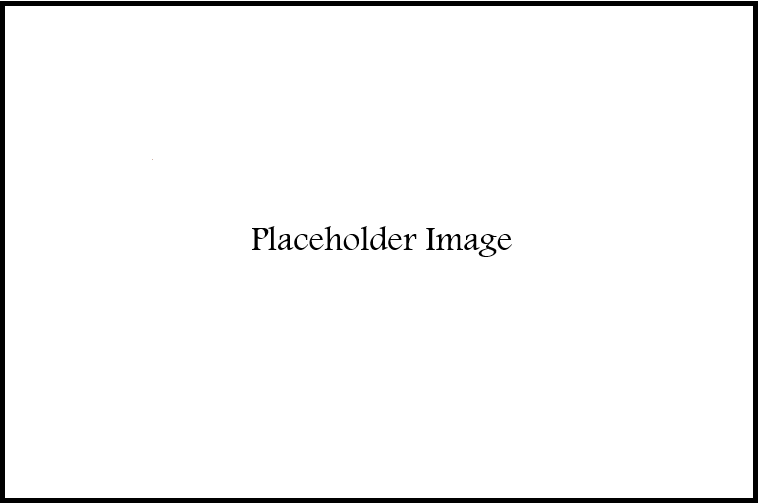
\includegraphics[width=0.75\linewidth, keepaspectratio]{figures/placeholder.png}
    \end{minipage}

    \vspace{\fill}
    \begin{flushright}
        \begin{spacing}{1}
            \textbf{
                \textcolor{coverBlue}{\LARGE{\detallesTrabajo}}\\
                \Large{\autorTrabajo}
                }\\
            \end{spacing}
        \end{flushright}

        \vspace{5 mm}
        \begin{flushright}
            \textcolor{coverBlue}{\large{Curso \cursoAcademico}}
        \end{flushright}

\end{titlepage}
\newpage

\pagenumbering{Roman}			    % roman page numbering 
\pagestyle{plain}				    % empty header, just page number in footer

\selectlanguage{spanish}

\setcounter{tocdepth}{3}		% define depth of toc
\tableofcontents				% display table of contents
\addcontentsline{toc}{section}{Índice General}

\listoffigures
\addcontentsline{toc}{section}{Índice de figuras}

\listoftables
\addcontentsline{toc}{section}{Índice de tablas}
%\newpage
% --------------------------
% Main matter
% --------------------------
\mainmatter
\pagenumbering{arabic}			% arabic page numbering
\setcounter{page}{1}			% set page counter
\pagestyle{fancy} 	            % fancy header and footer
\parskip=7pt                    % space after each paragraph
\parindent=0pt                  % suppress indentation of paragraphs


% !TEX root = ../main.tex
% called by main.tex
\chapter{Introducción al software CAD}
\label{ch:cad-intro}

\section {Autodesk Fusion}
Autodesk Fusion es un programa de diseño CAD integrado en la nube desarrollado por Autodesk. Este programa es donde se han desarrollado a día de hoy la mayoría de los diseños para el club de vuelo, ya que permite una integración rápida y ofrece una barrera de entrada a nuevos usuarios menor que otros softwares comerciales más extendidos en la industria (como CATIA V5). 
\par Las características por las que hemos elegido Fusion frente a otros son:
\begin{itemize}
    \item Es gratis, gracias a la cuenta de \texttt{alumnos.upm}
    \item Permite colaboración en la nube, evitando problemas de tranferencias de archivos
    \item Ofrece numerosos servicios, desde diseño paramétrico de componentes, hasta diseño de circuitos impresos o renderizado y animación.
    \item Por defecto cuenta con numerosas ayudas para nuevos usuarios que facilitan su introducción al CAD.
\end{itemize}

\subsection{Instalación de Fusion}
Esta parte está todavía en trabajo, me gustaría añadir una pequeña guía e imágenes del proceso. \todo{Instalación de Fusion}

\section{CATIA V5}
\newcommand{\catia}{CATIA V5 }
\catia es otro programa de diseño CAD mucho más arraigado en los sectores aeronáuticos e industrial, desarrollado por Dassault Systémes. En cuanto a las capacidades que ofrece, es un software muy potente, con una documentación muy extensa que permite aprender las funcionalidades más complejas a usuarios con el tiempo y la paciencia para buscarla. 
\par Un pequeño inconveniente de este software es que tiene tanta herencia (CATIA se desarrolló por primera vez en 1982) que no se ha decidido actualizar elementos fundamentales para facilitar la introducción de nuevos usuarios al CAD, como la interfaz de usuario, la funcionalidad o la distribución de los distintos entornos de trabajo. Siendo el objetivo de esta guía facilitar el diseño con la impresión 3D como fin, es importante recalcar que no recomiendo utilizar \catia como la entrada al diseño CAD, pero sí que será perfectamente adecuado para trabajar. 

\section{Prusa Slicer}
\todo{sección de PrusaSlicer}

\section{Ultimaker Cura}
\todo{sección de Cura}
% !TEX root = ../main.tex
% called by main.tex
\chapter{Particularidades de la Impresión 3D}\label{ch:3d-intro}

\section{Proceso de fabricación}
Para fabricar piezas impresas en 3D, es necesario de alguna manera, hacer llegar la información de la pieza a la impresora. Estas ``instrucciones'' son un código \texttt{GCODE}. Este tipo de códigos son un estándar utilizado para el control de máquinas herramientas de control numérico, una forma algo pomposa de describir una impresora 3D, pero es que el \texttt{GCODE} es el mismo código que utilizan las fresas o tornos CNC o máquinas de mecanizado por control numérico multieje. 
\par La obtención de estos códigos \texttt{GCODE} es muy sencilla. El proceso lo explicaré secuencialmente partiendo desde el programa de diseño 3D, hasta el momento de dar la orden a la impresora de fabricar la pieza. 

\subsection{De un diseño a una pieza real}
Teniendo por fin el diseño terminado, este no es más que una colección de ecuaciones que describen la geometría de la pieza. Para fabricarla, \textbf{exportaremos} este diseño como un archivo \texttt{.stl} o \texttt{.step/.stp}. Este tipo de archivos son un conjunto de triángulos en el caso del \texttt{.stl}, o un conjunto de ecuaciones en el caso del \texttt{.step/.stp} (esta vez estandarizado para ser comprensible para cualquier otro programa) que describen la geometría de la pieza. 
\par Ahora tenemos un archivo que es fácilmente comprensible para cualquier programa, no solo nuestro programa de diseño. Ahora, abriremos nuestro Slicer. En el slicer, deberemos elegir la orientación y la posición de la pieza en la cama de la impresora, así como algunos parámetros adicionales. Una vez satisfechos, solamente hay que hacer click en \textbf{slice} y el programa nos enseñará una previsualización de cómo quedará la pieza, mostrando las pasadas individuales del cabezal de la impresora.
\par Este archivo \texttt{GCODE} contendrá todas las instrucciones para la impresora, la temperatura a la que deberá calentar el cabezal, la cama, a dónde se tendrá que mover para cada deposición de filamento, etc. No hace falta entender nada de esto a más bajo nivel, ni siquiera es importante entender qué quieren decir las líneas dentro del archivo, no hace falta mirar dentro. Simplemente este archivo lo pasaremos a la impresora, guardándolo en la tarjeta micro SD de la impresora.
\todo{Añadir imágenes de la impresora, la tarjeta  y el lector del ordenador}. 
\par Finalmente, al introducir la tarjeta de nuevo en la impresora y encenderla, podremos navegar por los menús hasta seleccionar nuestro archivo \texttt{GCODE}. Al seleccionarlo, la impresora comenzará a imprimir la pieza.

\section{Importancia del Slicer}
Como se puede observar, el Slicer es una de las herramientas más poderosas en la impresión 3D, y un buen resultado dependerá tanto del diseño de la pieza, su geometría, como del Slicer. Esto es porque el Slicer tiene en cuenta una infinidad de parámetros, como las dimensiones de la impresora, las velocidades a las que se moverá, qué filamento estamos imprimiendo, qué temperaturas se utilizarán para ese filamento, etc. 
\par Generalmente, se utilizará la configuración predeterminada y ajustada a nuestra impresora, y no habrá que cambiar mucho estos ajustes. Por otro lado, para conseguir piezas más rígidas o más resistentes, en muchas ocasiones es suficiente con cambiar ajustes del Slicer y no es necesario rediseñar la geometría de la pieza. 
\par Es importante recalcar que con la experiencia y el uso, hemos conseguido encontrar en el club de vuelo una serie de ajustes para el Slicer que nos permiten conseguir impresiones rápidas, de una resistencia más que suficiente y con un nivel de detalles perfectamente adecuado para todos nuestros diseños. Por otro lado, si una pieza requiere una configuración muy particular de los ajustes del Slicer, el diseño de la propia pieza se deberá hacer con todo esto en cuenta. 

\section{Anisotropía de las piezas}
Por la propia naturaleza de la impresión 3D, es importante considerar cuál será el funcionamiento de las piezas, y a qué tipo de esfuerzos estarán sometidas. Esto nos permitirá elegir en qué orientación sería preferente imprimirlas. 

\par Debemos tener en cuenta que las piezas son mucho más susceptibles a romper bajo esfuerzos de tracción o pelado perpendiculares a los planos de las capas. Por ello hay que elegir una orientación que coloque los esfuerzos de tracción en el plano de las capas, como se puede observar en la \autoref{fig:fallo-traccion}. Sin embargo, las piezas impresas en 3D  funcionan mejor a compresión perpendicular al plano de las capas que en el plano. 

\begin{figure}[ht]
    \centering
    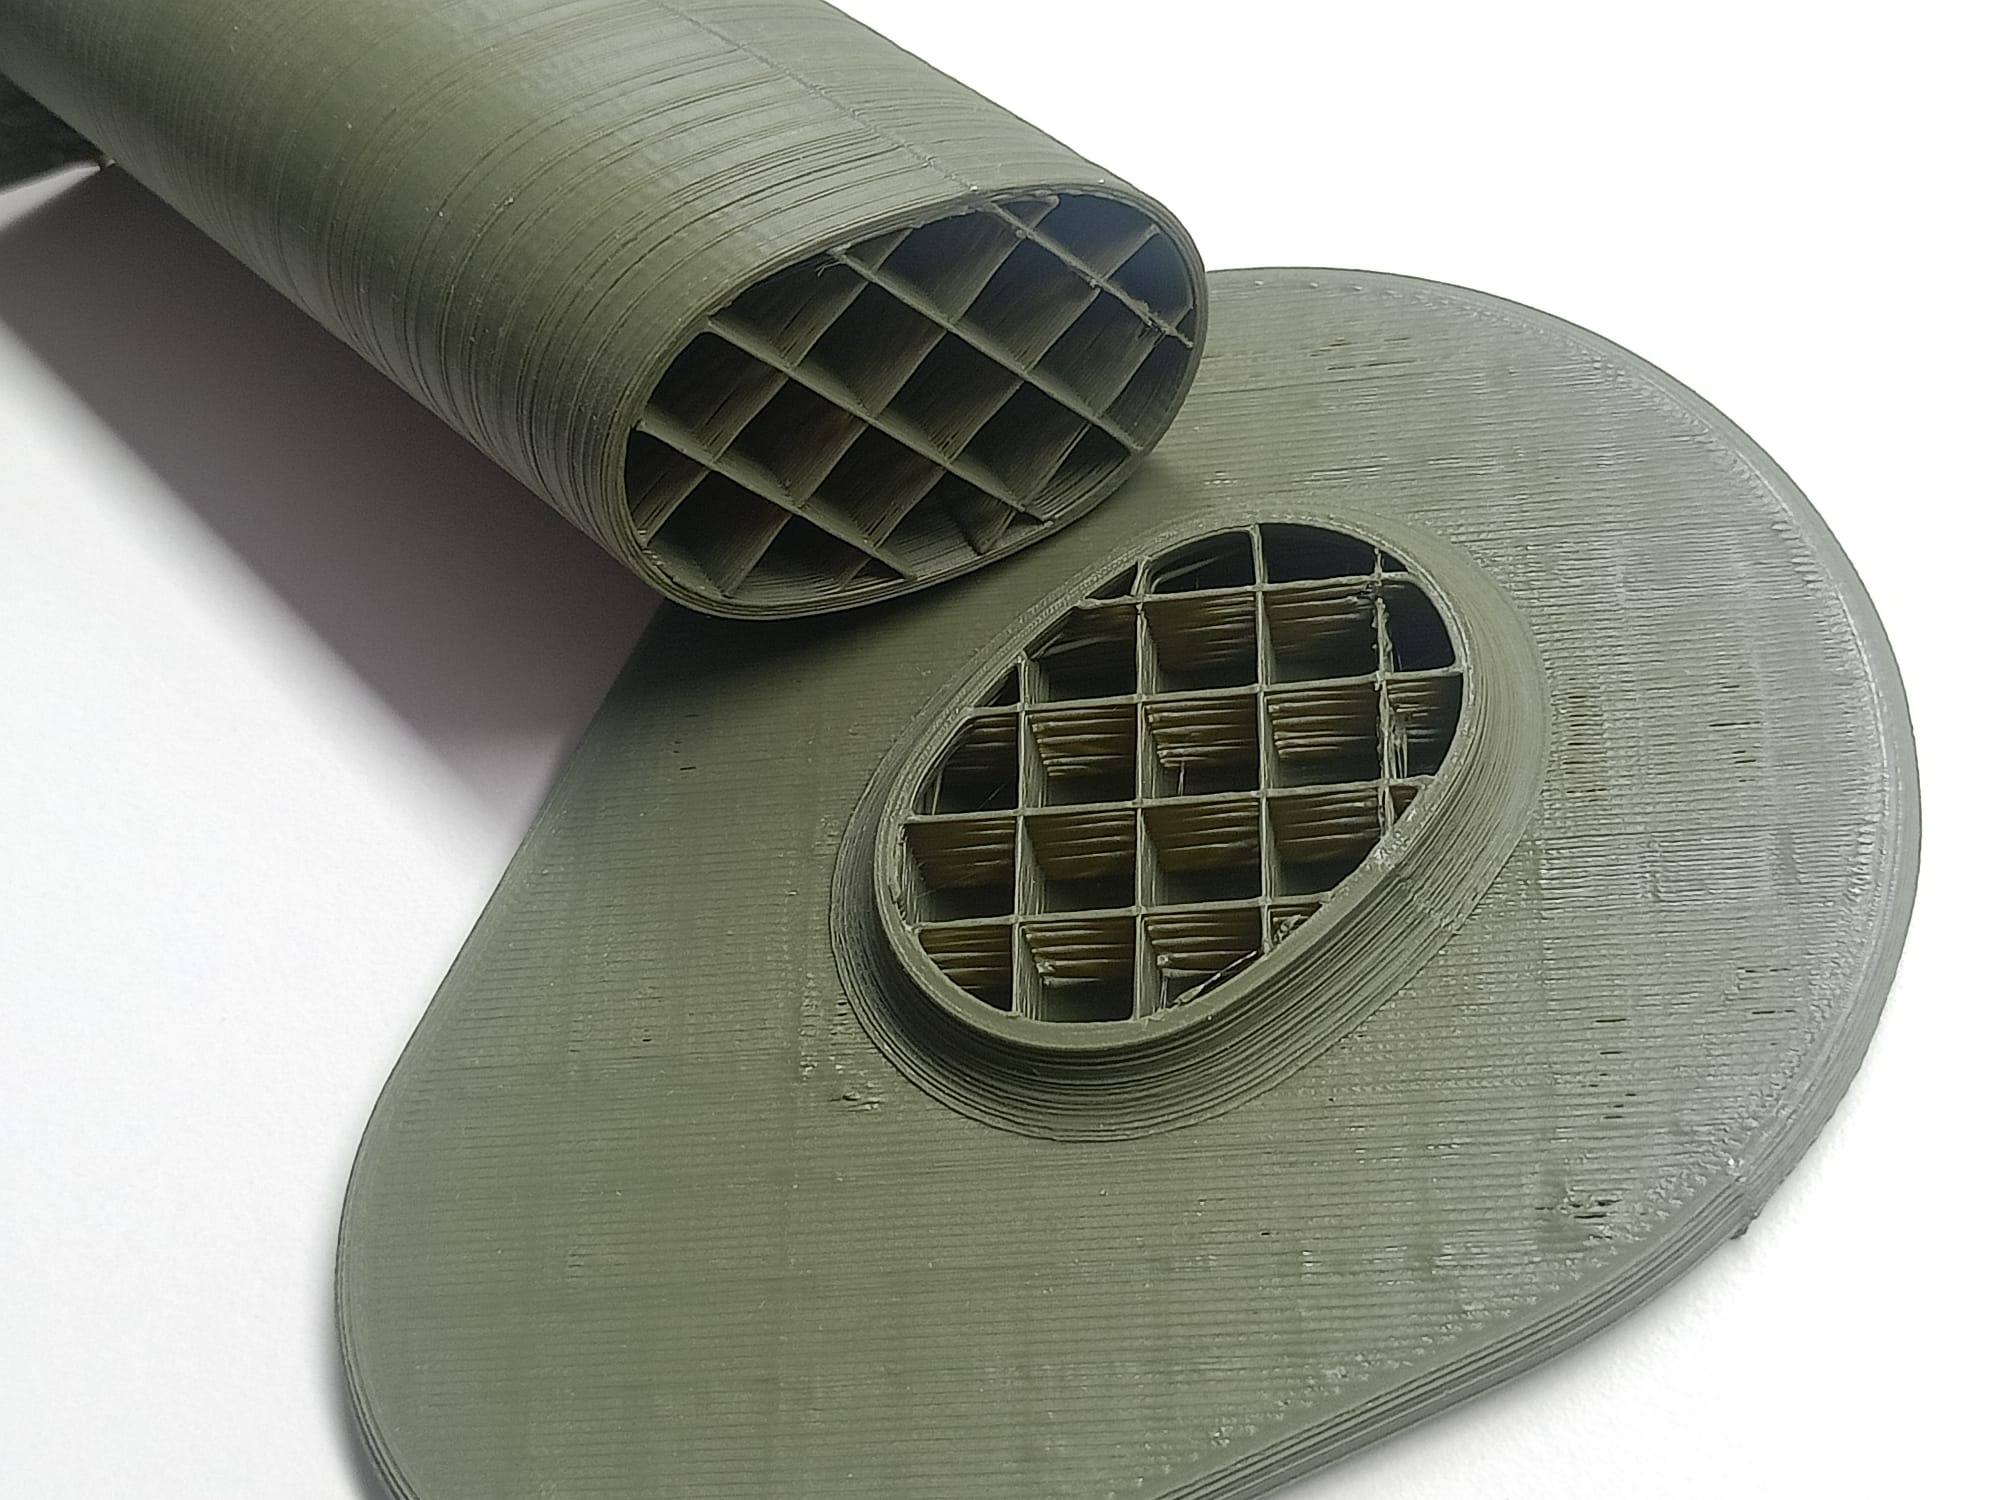
\includegraphics[width=0.5\textwidth]{figures/fallo-traccion.jpg}
    \caption{Ejemplo de un fallo por tracción en la dirección perpendicular a las capas}
    \label{fig:fallo-traccion}
\end{figure}
\todo{Añadir más imágenes de fallos en piezas impresas}

\section{Enfriamiento de las piezas}
Otro de los factores que más pueden conducir a error es no considerar, en piezas con cambios muy importantes en la sección, el enfriamiento desigual de la pieza.
\par El filamento es calentado hasta a unos 200\textdegree{}C típicamente para ser impreso, e inmediatamente después es enfriado hasta su temperatura de transición vítrea ($\approx 180$\textdegree{}C) al salir por la boquilla de la impresora. Una vez ha sido depositado, continúa enfriándose lentamente hasta la temperatura del resto de la pieza, que serán unos 60\textdegree{}C. Los gradientes térmicos que se presentan en estas situaciones son muy significativos, y el plástico experimentará expansiones y sobre todo, contracciones térmicas al ir reduciendo su temperatura. 
\par El enfriamiento genera esfuerzos internos en la pieza, generarán tracción en la dirección en la que el filamento haya sido depositado, pudiendo llegar a combar las piezas planas si la adherencia a la cama de la impresora no es suficiente.
\par Este tipo de problemas está agravado por el hecho de que la adherencia del PETG al vidrio (el material con el que más se imprime en el Club de Vuelo y el material de la cama de nuestra impresora) es muy baja. Es por esto que es tan importante utilizar la laca de la impresora generosamente, o conseguir un fleje metálico y texturizado para colocar en la cama. 
% !TEX root = ../main.tex
% called by main.tex
\chapter{Generalidades para el diseño}\label{ch:cad-recommendations}

\section{Puentes y geometría no soportada}
Durante el diseño de numerosas piezas, es muy frecuente encontrarse en una situación donde la geometría requiere voladizos. Estos requisitos pueden ser de origen estructural, garantizando que la orientación de las capas va a ir según los esfuerzos, estéticos, o simplemente porque la única orientación en la que la pieza se puede imprimir es con voladizos.
\par La primera recomendación a la hora de diseñar este tipo de características en una pieza \textbf{es evitarlas}. Sin embargo, por los motivos explicados anteriormente, es posible que no quede más remedio. En esos casos, se presentan a continuación algunas formas de conservar las características y asimismo mejorar la geometría para una impresión más eficiente.

\subsection*{Añadir un chaflán al voladizo}
Una de las mejores formas de facilitar la impresión de estas características es evitando el voladizo (desde el punto de vista de la impresora). Esto se puede conseguir añadiendo material de forma gradual para construir la plataforma sobre la que se irán depositando las capas del voladizo. De esta forma, se evita la necesidad de material de soporte, optimizando la impresión de las piezas. Esta geometría se puede conseguir muy fácilmente con un redondeo de los bordes o un chaflán.

\begin{figure}[ht]
	\centering
	
\includegraphics[width=0.6\linewidth]{figures/chaflan.pdf}
	\caption{Ejemplo de cómo un redondeo permite la impresión de un voladizo}
	\label{fig:overhang-idea}
\end{figure}

\subsection*{Soportar el voladizo en ambos extremos}
Si se busca conseguir un ``techo,'' se pueden mejorar notablemente los resultados al soportar el mismo en los dos extremos, especialmente si se aplican las sugerencias de la sección anterior y se añaden chaflanes (o \textit{fillets}). De esta forma, la distancia que será impresa sin soporte será lo menor posible, siempre que el resto de restricciones de diseño lo permitan.

\begin{figure}[ht]
	\begin{subfigure}[t]{0.49\textwidth}
		\centering
		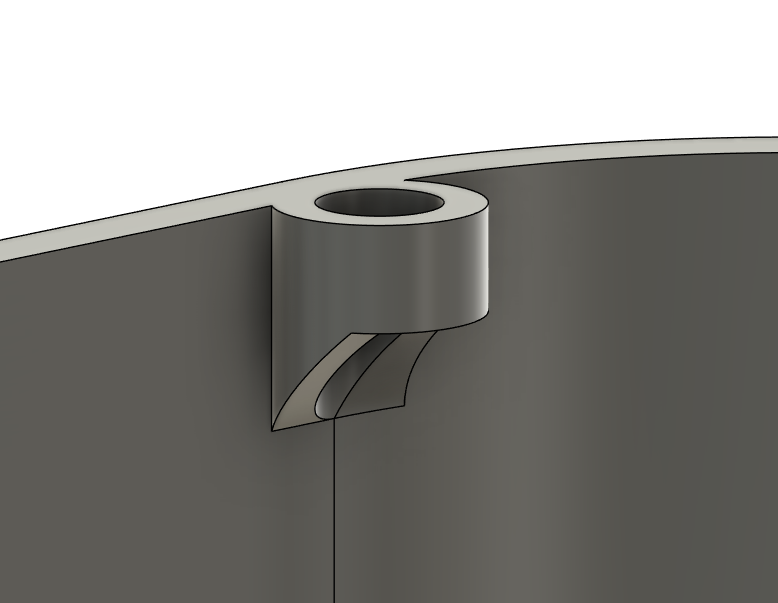
\includegraphics[width=\linewidth]{figures/chaflan.png}
		\caption{Ejemplo de un chaflán en geometría de fijación}
		\label{fig:fusion-chaflan}
	\end{subfigure}
	\hfill
	\begin{subfigure}[t]{0.49\textwidth}
		\centering
		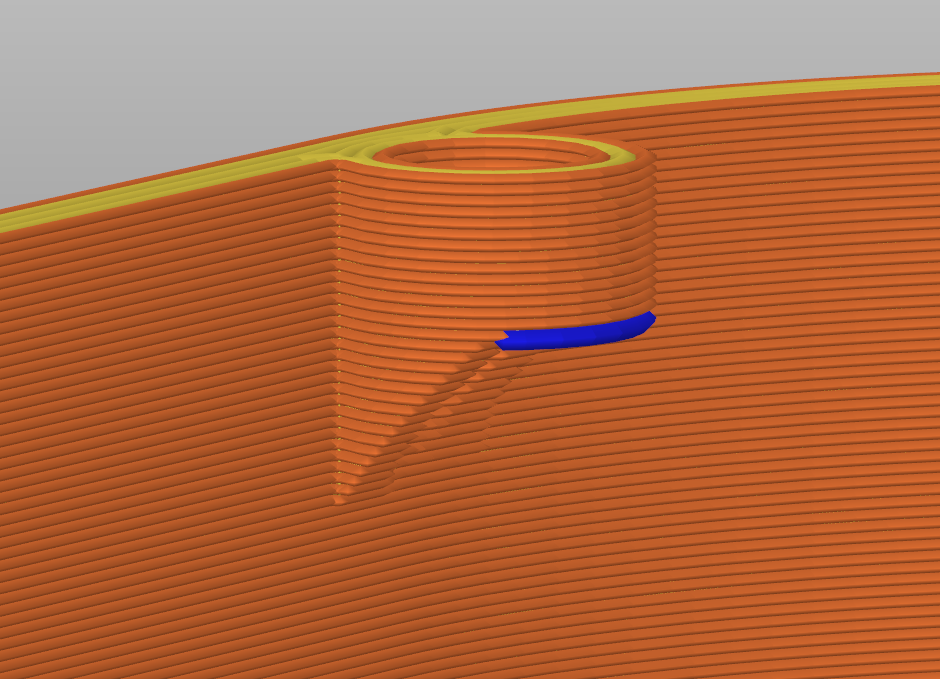
\includegraphics[width=\linewidth]{figures/chaflan-prusa.png}
		\caption[GCODE de un chaflán en un voladizo]{GCODE de un chaflán en un voladizo. En azul se puede observar donde se sigue imprimiendo sin soportes}
		\label{fig:prusa-chaflan}
	\end{subfigure}
\end{figure}

\section{Piezas o partes de piezas estructurales}
En muchas ocasiones, sobre todo en diseños mecánicos, habrá piezas de responsabilidad estructural para el correcto funcionamiento del diseño. En estos casos, es fundamental entender el recorrido de las cargas, dónde podrá haber concentraciones de esfuerzos y retocar el diseño funcional de la pieza para poder reforzar estos aspectos.

\subsection{Cargas en un plano}
Cuando el diseño permite conocer de antemano que las cargas a las que una pieza va a estar sometida estarán contenidas en un plano, (tracción-compresión, cortantes, etc.), lo más recomendable en  la mayoría de los casos es contener todos estos esfuerzos en el plano. Por ejemplo, con un engranaje muy solicitado, como el de la \autoref{fig:engranaje-cargas}
\begin{figure}[ht]
	\centering
	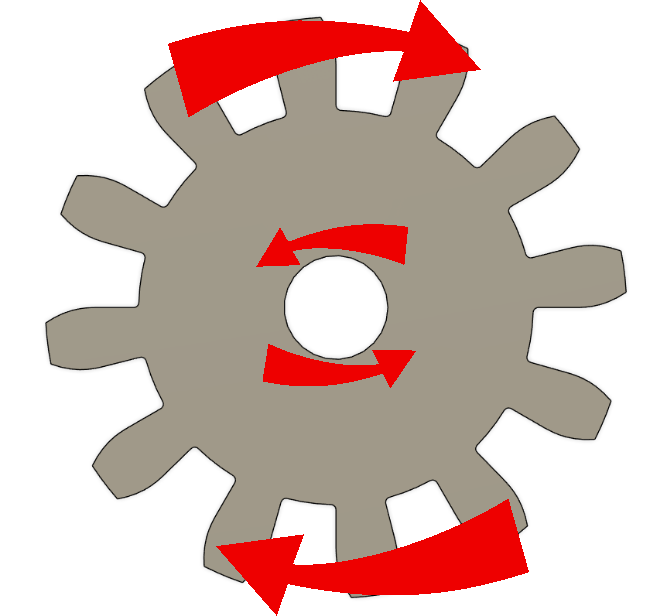
\includegraphics[width=0.5\textwidth]{figures/engranaje.png}
	\caption{Diseño de un engranaje con la previsión de las cargas}
	\label{fig:engranaje-cargas}
\end{figure}

El el caso de que sea necesario aumentar la resistencia en el plano de la pieza, una de las mejores recomendaciones es conseguir más perímetros en las direcciones de la carga. En el caso del engranaje, por contra-intuitivo que parezca, haciendo un patrón de agujeros como el de la \autoref{fig:engranaje-rediseño} puede aumentar la resistencia a fallos en el plano.
\begin{figure}[ht]
	\centering
	\begin{subfigure}[b]{0.49\textwidth}
		\centering
		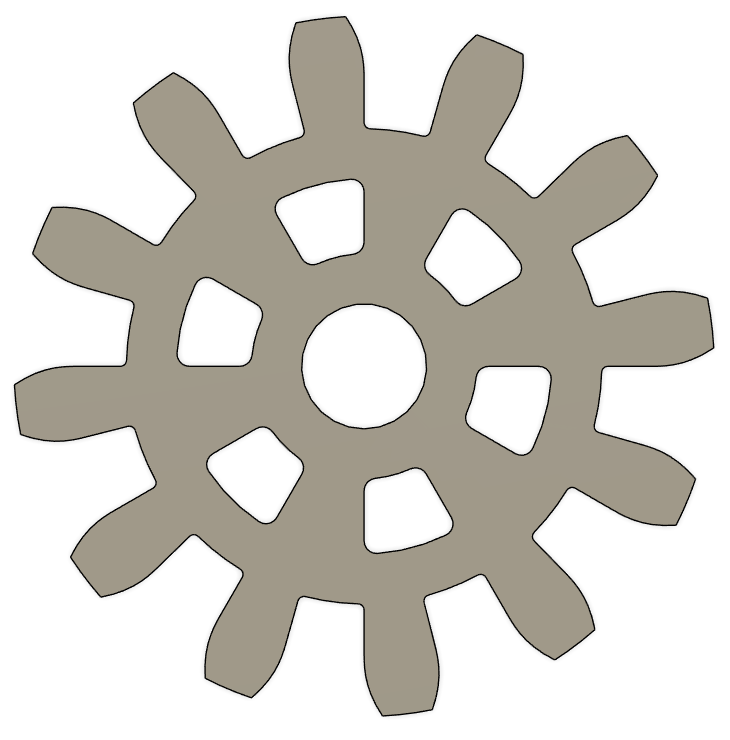
\includegraphics[width=\linewidth]{figures/engranaje-agujeros.png}
		\caption{Rediseño del engranaje para mejorar la resistencia}
		\label{fig:engranaje-agujeros}
	\end{subfigure}
	\hfill
	\begin{subfigure}[b]{0.49\textwidth}
		\centering
		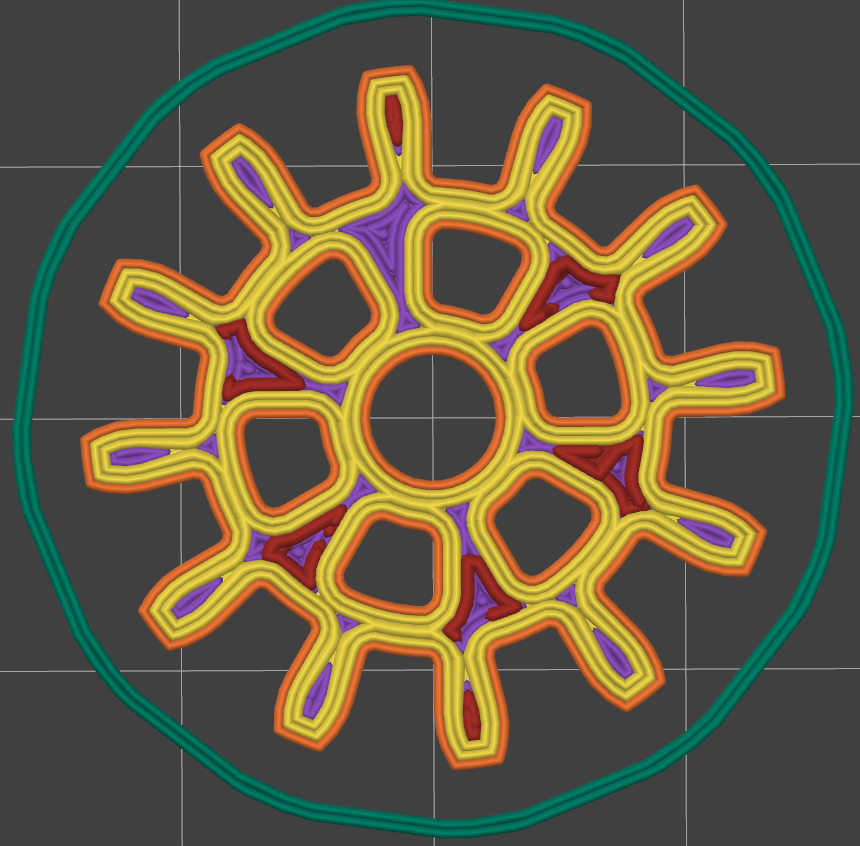
\includegraphics[width=\linewidth, angle=90]{figures/engranaje-agujeros-slice.png}
		\caption{Vista del GCODE}\label{fig:engranaje-agujeros-slice}
	\end{subfigure}
	\caption{Rediseño del engranaje}\label{fig:engranaje-rediseño}
\end{figure}

\section{Ejes y montajes con tolerancias estrechas}
Continuando con el tema de diseños mecánicos donde va a haber movimiento entre piezas, van a ser fundamentales los ``ejes'' y los montajes con tolerancias.
\par Detallar los procedimientos para diseño de este tipo de mecanismos es algo mucho más complejo de lo que esta guía pretende abarcar, incluso sin tener en cuenta que esto debe ser para piezas optimizadas para la impresión 3D. En su defecto, se proponen a continuación una serie de guías interesantes para asistir con el diseño funcional de estas piezas.

\subsection{Ejes no impresos}
En primer lugar, una de las mejores recomendaciones es considerar utilizar ejes no impresos, ya que los materiales metálicos (acero, o aluminio) en el formato de barras redondas (mecanizadas o extruidas), son baratos y accesibles, y su inclusión en los diseños puede mejorar notablemente el funcionamiento y la resistencia del producto final.
\par Sin embargo, la utilización de ejes no impresos en mecanismos de grandes solicitaciones implica otro tipo de consideraciones, entre ellas:
\begin{itemize}
	\item Correcta orientación de las capas en las piezas que interactúan con el eje
	\item Posible desgaste por fricción de las piezas que interactúan con el eje
	\item Montaje del conjunto
\end{itemize}
De todas las anteriores, probablemente la consideración más importante es la del montaje, ya que utilizar una pieza más para el eje es añadir complejidad al conjunto. Al diseñar esto, se debe asegurar que el montaje es posible, aunque se complique de forma notable.

\subsection{Montajes con tolerancias estrechas}
Para este tipo de montajes, el mejor consejo es el siguiente: evitarlos. Cuando se deben montar varias piezas con tolerancias estrechas, debido a las irregularidades de la impresión 3D, se busca que los montajes queden clasificados como montajes con `interferencia'. Esto quiere decir que dos piezas, en sus dimensiones nominales, compartirán un espacio y tiempo (lo que debería ser imposible si no hubiera deformación). Para mejorar este tipo de uniones o montajes, la recomendación es añadir mecanismos flexibles a las piezas que permitan acomodar las posibles variaciones en las dimensiones de los elementos del montaje. \todo{añadir imágenes ilustrativas de montajes `flexibles'}
\par La idea con la que el diseño se debe realizar es que si en lugar de querer montar las piezas perfectas del software CAD, se montaran algo un poco más ``amorfo'', todo vaya bien porque las piezas son flexibles \textbf{donde importa}.

\subsection{Agujeros}
Este tipo de geometría, cuando es funcional, no necesita mucha especificación. No obstante, es interesante mencionar los fallos más típicos que se pueden dar, sobre todo para la interacción entre varias piezas.
\par Los agujeros se suelen deformar cuando se imprimen en la dirección perpendicular a las capas. Una recomendación sería incluir, cuando la precisión dimensional sea necesaria, modificaciones en el propio diseño del agujero, para que este no sea exactamente circular sino que el ángulo del saliente esté limitado.

\begin{figure}[ht]
	\centering
	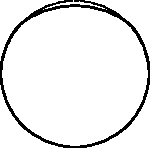
\includegraphics[width= 0.20\linewidth]{figures/agujero-rediseño.pdf}
	\caption{Muestra de cómo puede quedar un agujero habiendo aplanado la parte superior.}
	\label{fig:agujero-rediseño}
\end{figure}

\subsection{Juntas en Cola de Milano}
Este tipo de juntas son geniales para conseguir montajes rápidos e inequívocos (si se utilizan correctamente). \todo{añadir foto de junta en cola de milano, explicar cómo hacerla asimétrica.} Su principal función es la unión rígida de componentes, teniendo en cuenta que la versión más básica de esta unión no soportará cargas en una dirección (la que desmontaría la junta).

\section{Piezas planas o placas}
A la hora de imprimir piezas planas o placas, es muy importante considerar si es realmente necesario imprimirlas. En la mayoría de los casos, las piezas con esta geometría se pueden diseñar para tener unos requisitos dimensionales menos estrictos y poder ser fabricada mediante otros métodos (como en madera con taladros).
\par No obstante, puede ser interesante imprimir en 3D plantillas para la fabricación de estas piezas (un localizador para los agujeros, por ejemplo).

%% !TEX root = ../main.tex
% called by main.tex
\chapter{Análisis de la defectología}\label{ch:defectology}

En esta parte quiero dedicar un espacio a comentar algunos de los defectos de impresión típicos. Con esto me refiero a cualquier anomalía, desde un mínimo artefacto imprevisto en la pieza final, a fallos en la impresión. 

\section{Infra-extrusión o Sobre-extrusión}
\todo{Conseguir e incluir foto de sobre extrusión e infra-extrusión}\\
Este tipo de errores son más complicados de ver. Se pueden detectar en la capa superior de una impresión, donde el relleno se une con los perímetros, y se puede solucionar ajustando el multiplicador de extrusión (\texttt{Extrusion Multiplier}) en PrusaSlicer, en la dirección correcta. Si se ve sobre-extrusión, habría que reducirlo ligeramente, y si se ve infra-extrusión, habrá que aumentarlo ligeramente. Es importante comentar que este parámetro vale 1 por defecto, y que un filamento bien calibrado tiene el multiplicador de extrusión oscilando entre 0.94 y 1.04. Valores mayores o menores son indicativos de que el problema es otro.  

\section{Perímetros externos primero}

\section{Pie de elefante (Elephant's foot)}

\section{La pieza se levanta de la cama}

\section{Mal alineamiento de las capas}

%% ! TEX root = main.tex
\chapter{Referencias para Componentes concretos}
En esta parte se presentan tablas, dimensiones y planos de componentes frecuentes para facilitar el diseño de estas geometrías.

\section{Tuercas e Insertos Roscados}
En caso de que se quiera fabricar una unión roscada, en lugar de diseñar la rosca en el plástico, es más recomendable utilizar componentes metálicos para hacer las uniones. A continuación se presentan los tamaños típicos de tuercas ISO y para los insertos roscados disponibles en el club.

\subsection{Tuercas ISO 4033}
\begin{figure}[ht]
	\centering
	
\includegraphics[width=0.5\textwidth, trim={135mm, 90mm, 115mm, 97mm}, clip]{figures/plano_tuerca.pdf}
	\caption{Dimensiones de referencia para las tuercas}\label{fig:plano-tuerca}
\end{figure}

\begin{table}[ht]
	\centering
	\caption{Dimensiones de las tuercas ISO 4033}\label{tab:iso-4033}
	\begin{tabular}{|c|c|c|c|c|}
		\hline
		\textbf{Métrica} & \textbf{Paso} & \textbf{e [mm]} & \textbf{m [mm]} & \textbf{s [mm]} \\
		\hline
		\hline
		M2               & 0.4           & 4.38            & 2               & 4               \\
		M2.5             & 0.45          & 5.51            & 2.5             & 5               \\
		\hline
		M3               & 0.5           & 6.08            & 3               & 5.5             \\
		M4               & 0.7           & 7.74            & 4               & 7               \\
		\hline
		M5               & 0.8           & 0.87            & 5               & 8               \\
		M6               & 1             & 11.05           & 6               & 10              \\
		\hline
		M8               & 1.25          & 14.38           & 8               & 13              \\
		M10              & 1.5           & 18.9            & 10              & 17              \\
		\hline
		M12              & 1.75          & 21.1            & 12              & 19              \\
		M14              & 2             & 24.49           & 14              & 22              \\
		\hline
		M16              & 2             & 26.375          & 16              & 24              \\
		M18              & 2.5           & 30.14           & 18              & 27              \\
		\hline
	\end{tabular}
\end{table}

\subsection{Insertos Roscados}
\begin{figure}[ht]
	\centering
	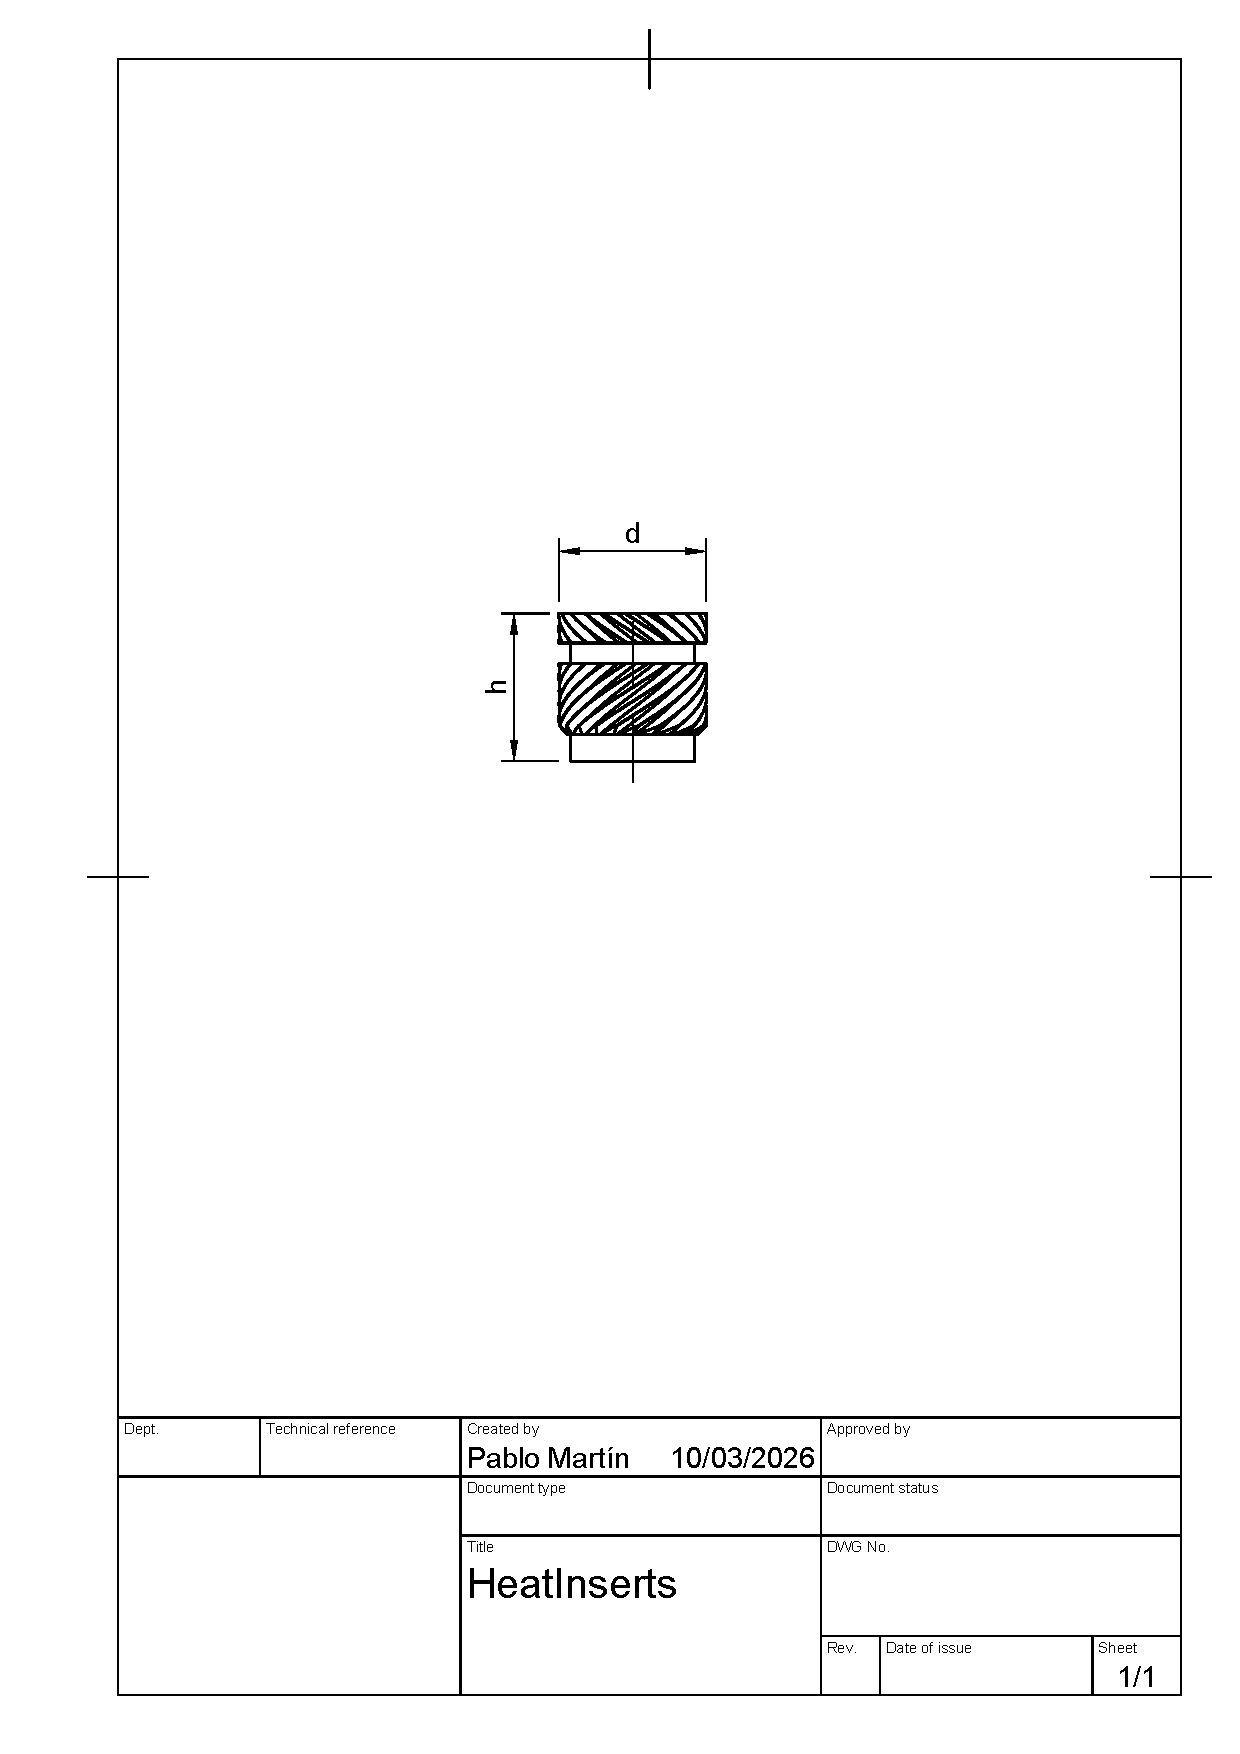
\includegraphics[width=0.5\textwidth, trim={60mm, 160mm, 60mm, 85mm}, clip]{figures/plano-inserto.pdf}
	\caption{Dimensiones relevantes para los insertos roscados}\label{fig:plano-inserto}
\end{figure}


%\include{cuerpo/chapter6}

% --------------------------
% Back matter
% --------------------------
%\backmatter
\listoftodos
\bibliographystyle{IEEEtranSpa}
%\cleardoublepage
\phantomsection
%\addcontentsline{toc}{chapter}{Referencias}
%\bibliography{references}

\appendix
\setcounter{secnumdepth}{2} %Reactiva la numeración para los anexos
\selectlanguage{spanish}
%\include{anexos/anexo1}
%\include{anexos/anexo2}

% ==================================================
% End of document
% ==================================================
\end{document}
